%   *** The Essential Emacs Hotkey ***
%(defun run-latex () (interactive) (progn (TeX-save-document (TeX-master-file)) (TeX-command "LaTeX" (quote TeX-master-file) -1)))
%(DefGlobKey "H-a" 'run-latex)

\documentclass[a4paper,11pt]{article}

\pagestyle{plain}
\usepackage{url}
\usepackage[pdftex]{graphicx}
\usepackage{fancyvrb}
\usepackage{wrapfig}
\usepackage{epsfig}

\newcommand{\nnf}[1]{\mathsf{NNF} #1}
\newcommand{\tilda}{$\sim$}
\newcommand{\dom}[1]{\mathsf{dom} #1}
\newcommand{\fv}[1]{\mathsf{FV} #1}
\newcommand{\bold}[1]{\textbf #1}
\newcommand{\andrew}[1]{\texttt{#1}}
\newcommand{\comm}[1]{ \begin{comment} #1 \end{comment} }

%needed for \begin{comment}
\usepackage{verbatim}

%needed for just about everything
\usepackage{amsmath}

%needed for \theoremstyle{...}
\usepackage{amsthm}

%needed for \mathbb, \mathcal etc.
\usepackage{amssymb}
\usepackage{amsfonts}

%\usepackage{pdflatex}
%\usepackage{pdfcolor}
%\usepackage{psticks}

\usepackage{latexsym}
\usepackage[latin1]{inputenc}

%needed for \mathscr
%\usepackage{mathrsfs}

%funks up \mathcal
%\usepackage{eucal}

\title{Proof Objects for Logical Translations}

\author{Andrew Polonsky\quad\quad\quad Marc Bezem\\\\
Department of Informatics\\University of Bergen\\Norway}
\date{}

\begin{document}

\theoremstyle{plain} 
\newtheorem{thm}{Theorem}
\theoremstyle{definition}
\newtheorem{dfn}[thm]{Definition}
\newtheorem{ex}[thm]{Example}
\newtheorem{fact}[thm]{Fact}
\maketitle

\begin{abstract}
\noindent
One principal obstacle to integrating into Coq the full power
of automated theorem provers is translation of the input into
the prover's internal logic.  Many translations introduce new
predicates which actually change the logical meaning,
making it difficult to recover a proof object of
the input problem from the solution to the translated problem.
We present a novel method for translating back proofs by
reinterpreting the new predicates.  The method is described
for a particular prover logic, but is in principle generic.  We
illustrate the idea by a few examples in Coq.  Since
Coq allows abstraction over the new predicates, the proofs
can be obtained with minimal overhead.

\end{abstract}

\section{Introduction}

Coq is a great interactive theorem prover. Yet as of today, complete
formalization of complex results requires considerable amount of effort.  Many small
steps which would be left out of a published proof have to be explicitly justified
by the user.  In contrast, automated theorem provers can solve small problems
completely autonomously, but are inherently incapable of 
dealing with deep mathematical results.  If it were possible to integrate
the automated First-Order Logic (FOL) provers into the Coq system, 
the amount of detail to be
spelled out in formalizing a theorem would be greatly reduced.

The major obstacle to this enterprise is the fact that 
the resolution method, which is the basis of most high-performance FOL provers
today, necessarily involves a normalization step converting the original problem into a
Clause Normal Form, see \cite[pp.19--99,273--333]{HandbookAR}.  
This step is difficult to undo at the level of proof
objects.  Skolemization in particular makes it difficult to lift the proof of the
translated problem to a lambda term inhabiting the type of the original problem.

\newpage
We present a translation with proof objects for Coherent Logic (CL), which extends resolution 
with existential quantifiers, making skolemization unnecessary.  The Geo2007 prover
is an example of an automated theorem prover based on Coherent Logic competing in CASC 
\cite{CASC:06}.  Our central result is that the proof objects
for the input problem can be recovered from the proof of the translation with
virtually no effort.

\section{Coherent Logic}

The general form of a coherent formula is 
\begin{equation}
A_1 \land \cdots \land A_m \to
B_1 \lor \cdots \lor B_n
\end{equation}
with $A_i$ atomic and $B_i$ of the form
\[\exists \vec y. D_1 \land \cdots \land D_k\]
with $D_i$ atomic.  In contrast with resolution, where $B_i$ must also be atoms,
coherent logic allows $B_i$ to be existentially quantified conjunctions of atoms.
If the clause (1) contains free variables, these are implicitly 
universally quantified.  Thus coherent clauses are interpreted as 
universal closures of (1).

One of the attractive features of Coherent Logic is that, in a sense, it is its
own proof theory.  Specifically, a set of coherent clauses serves both as a set of
axioms as well as a complete set of deduction rules which generate all logical
consequences of these axioms.  

\begin{dfn} \label{clAxs}
Let $\Gamma$ be a set of facts (atomic formulas).  
$\Gamma$ can be viewed as a coherent theory by
taking the set
%\[\{\top \to A \mid A \in \Gamma \}\]
\[\{\top \to A\}_{A \in \Gamma}\]
\end{dfn}

Generally, $\top$ will be written on the left of the arrow in (1) to denote 
that $m=0$.  If $n=0$, we will write $\bot$ on the right.  

\begin{dfn} \label{clPrv}
Let $\Gamma$ be a set of closed facts, $\mathcal T$ a coherent theory,
$\phi$ a fact.  Let $\dom(\Gamma)$ denote the set of terms which occur in
$\Gamma$. The relation $\Gamma \vdash_{\mathcal T} \phi$ is defined by induction:
\begin{description}
\item{\bf Base} 
$\Gamma \vdash_{\mathcal T} \phi$ if $\phi \in \Gamma$.
\item{\bf Induction}
Let $C = \bigwedge A_i \to \bigvee B_j$ be a clause in $\mathcal T$
and ${\sigma : \fv (C) \to \dom(\Gamma)}$\\
a substitution with
$\{A_i^\sigma\}_{1\leq i\leq m} \subseteq \Gamma$.
If for each $1\leq j\leq n$,\\ 
$B_j = \exists \vec y. D_1 \land \cdots \land D_k$ we have
$\Gamma \cup \{D^\sigma_i\}_{1\leq i\leq k} \vdash \phi$, 
then $\Gamma \vdash \phi$.
\end{description}
With no loss of completeness, we will restrict our attention to \emph{ground} reasoning.
This means that all of the facts in $\Gamma$ are closed and in the induction step
the existentials introduce fresh constants into the $D^\sigma_i$.
\end{dfn}

\begin{figure}
\begin{minipage}[b]{0.5\linewidth}
\centering
\scalebox{0.7}{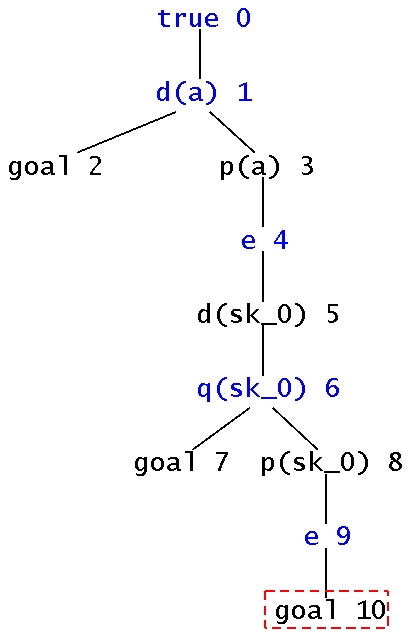
\includegraphics{ex1.jpg}}
\caption{A derivation of $goal$}
\label{fig1}
\end{minipage}
\begin{minipage}[b]{0.5\linewidth}
\centering
\begin{math}
\begin{array}{r c l}
\lnot \lnot \phi & \longrightarrow & \phi\\
\lnot \bigwedge \phi_i & \longrightarrow & \bigvee \lnot \phi_i \\
\lnot \bigvee \phi_i & \longrightarrow & \bigwedge \lnot \phi_i \\
\lnot \exists \vec x \phi & \longrightarrow & \forall \vec x \lnot \phi\\
\lnot \forall \vec x \phi & \longrightarrow & \exists \vec x \lnot \phi\\
(\phi \to \psi) & \longrightarrow &(\lnot \phi \lor \psi)\\
(\phi \leftrightarrow \psi) & \longrightarrow 
&(\phi \land \psi) \lor (\lnot \phi \land \lnot \psi)\\\\
\end{array}
\end{math}
\caption{NNF transformation}
\label{nnf}
\end{minipage}
\end{figure}

\begin{ex}
Coherent derivations are usually visualized as trees.  For example, consider
the theory
\[ \mathcal T = \left\{
\begin{array}{r r l}
\top &\to &d(a)\\
\forall x.\quad d(x) &\to &goal \lor (p(x) \land E)\\
E &\to &\exists y. (q(y) \land d(y))\\
\forall x.\quad p(x) \land q(x) &\to &goal
\end{array}
\right.
\]
Then $\emptyset \vdash_{\mathcal T} goal$.  The derivation as per Definition~\ref{clPrv}
is illustrated in Figure~\ref{fig1}.  Every node in the tree corresponds to a state
$\Gamma$ consisting of all the facts occurring on the path from the root to the node. 
Inference nodes (0,1,4,6, and 9) correspond to applications of the induction case of 
$\vdash_{\mathcal T}$,
while the leaves correspond to the base case.  See \cite{FishBez09} for a detailed
discussion.
John Fisher implemented the ``visual'' prover which we used to generate the trees.
\end{ex}

\begin{fact}[Completeness of Coherent Logic, \cite{Beze:Coqu:05}]
Let $\mathcal T$ be a coherent theory, $\phi$ a closed atomic formula.  Then
\[\emptyset \vdash_{\mathcal T} \phi \iff \mathcal T \models \phi\]
where $\models$ is the Tarskian entailment of $\mathcal T$ as a first-order theory.
\end{fact}

\section{The Canonical Translation}

The basic idea for a translation from FOL to CL was suggested in \cite{Beze:Coqu:05}. 
Essentially it consists of encoding the semantic tableaux proof method 
\cite[pp.100--178]{HandbookAR} into a set of coherent clauses.  A refutation of the 
given formula
by a tableaux system corresponds to a derivation of $\bot$ from the translated
theory by a CL prover.

Although general tableau rules for logical operators come in both polarities, 
we will find it convenient to restrict ourselves
 only to the positive rules.  As such, we will consider \emph{negation
normal forms} (NNFs) as the basic forms of input, where negations only occur in
front of atomic formulae and the only propositional connectives are $\land$ and $\lor$.
A general FOL formula is converted into a NNF by normalizing it under
the rules in Figure~\ref{nnf}.

\newpage
We now define the canonical translation from FOL to CL.
\begin{dfn} \label{nnfxl}
Let $P$ be a formula in NNF.
\begin{itemize}

\item
For an atomic predicate $A$ occuring in $P$, let
\begin{itemize}
\item
$T_A$, $F_A$ be fresh predicate symbols of the same arity as $A$,
\item
$C_A$ be the coherent clause
\[\forall \vec x. \quad T_A(\vec x) \land F_A(\vec x) \to \bot\]
\end{itemize}

\item
For a literal $L \subseteq P$, define the formula
\[L^t = 
\begin{cases} 
T_A(\vec{\,t}\,) & \qquad \text{if $L = A(\vec{\,t}\,)$}\\
F_A(\vec{\,t}\,) & \qquad \text{if $L = \lnot A(\vec{\,t}\,)$}
\end{cases}
\]

\item
For a compound (non-literal) subformula $Q \subseteq P$, let
\begin{itemize}
\item
$T_Q$ be a fresh predicate of arity $|\fv (Q)|$,
\item
$Q^t$ be the formula $T_Q(\vec x)$, where $\vec x = \fv (Q)$,
\item
$C_Q$ be the coherent clause defined according to the top connective in $Q$,
with implicit universal quantification over all free variables:
\large{
\[
\begin{array}{c|l}
Q &\multicolumn{1}{c}{C_Q=\forall \vec x.\underline{\qquad\qquad}}\\
\hline
\\Q_1 \land Q_2 \land \cdots \land Q_n &
Q^t \to Q^t_1 \land Q^t_2 \land \cdots \land Q^t_n \\
\\Q_1 \lor Q_2 \lor \cdots \lor Q_n &
Q^t \to Q^t_1 \lor Q^t_2 \lor \cdots \lor Q^t_n \\
\\\exists \vec{y} R&
Q^t \to \exists \vec{y} R^t\\
\\\forall \vec{y} R &
Q^t \to R^t
\end{array}
\]
}
\end{itemize}

\item
The \emph{canonical coherent theory of P} is the set
\[\mathcal{T}_P = \{\top \to P^t\} ~\cup~ 
\{C_A\}_{A~\text{atomic predicate in}~P} ~\cup~ \{C_Q\}_{Q\subseteq P} 
\]

\end{itemize}
\end{dfn}

\begin{dfn} \label{clxl}
Let $\Gamma$ be a first-order theory.  The \emph{canonical translation} of
$\Gamma$ is
\[\mathcal{T}_\Gamma = \bigcup_{\phi \in \Gamma} \mathcal{T}_{\nnf (\phi)}\]
\end{dfn}

\begin{figure}
\begin{center}
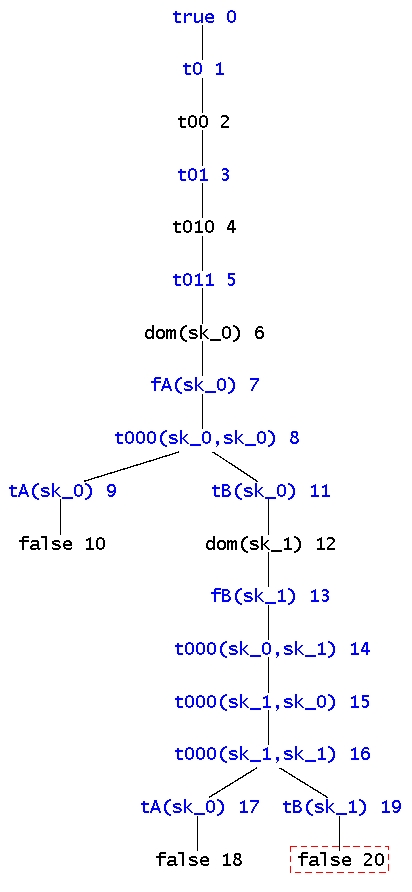
\includegraphics{ex2.jpg}
\end{center}
\caption{A derivation of {\bf false}}
\label{fig2}
\end{figure}

\begin{ex} \label{xlex}
Suppose we wish to find a coherent theory equisatisfiable with the formula
\[\phi = \lnot ((\forall x y. Ax \lor By) \to (\forall x. Ax) \lor (\forall x. By))\]

The first step is to compute the negation normal form of $\phi$:
\[\nnf(\phi) = (\forall x y. Ax \lor By) 
\land (\exists x. \lnot Ax \land \exists y. \lnot By)\]

Now the new predicates $T_\psi$ for every $\psi \subseteq \nnf(\phi)$ 
are introduced:\\
$T_{(\forall x y. Ax \lor By) \land (\exists x. \lnot Ax \land \exists y. \lnot By)}$,
$T_{\forall x y. Ax \lor By}$, $T_{\exists x. \lnot Ax \land \exists y. \lnot By}$,
$T_{Ax \lor By}(x,y)$, $T_{\exists x. \lnot Ax}$, $T_{\exists y. \lnot By}$,
$T_A(x)$, $F_A(x)$, $T_B(x)$, $F_B(x)$.

Finally, one constructs the clauses as per Definition \ref{nnfxl}:
\[
\mathcal T_\phi = \left\{
\begin{array}{l l l}
\top &\to &T_{(\forall x y. Ax \lor By) 
\land (\exists x. \lnot Ax \land \exists y. \lnot By)}\\
T_{(\forall x y. Ax \lor By) \land (\exists x. \lnot Ax \land \exists y. \lnot By)} &\to
&T_{\forall x y. Ax \lor By} \land T_{\exists x. \lnot Ax \land \exists y. \lnot By}\\
T_{\forall x y. Ax \lor By} &\to &T_{Ax \lor By}(x,y)\\
T_{Ax \lor By}(x,y) &\to &T_A(x) \lor T_B(y)\\
T_{\exists x. \lnot Ax \land \exists y. \lnot By}
&\to &T_{\exists x. \lnot Ax} \land T_{\exists y. \lnot By}\\
T_{\exists x. \lnot Ax} &\to &\exists x. F_A(x)\\
T_{\exists y. \lnot By} &\to &\exists y. F_B(y)\\
T_A(v) \land F_A(v) &\to &\bot\\
T_B(v) \land F_B(v) &\to &\bot\\
\end{array}
\right.
\]
As the reader may have been expecting, the set of clauses
above is inconsistent.  The derivation of $\bot$ from $\mathcal T_\phi$ is
shown in Figure~\ref{fig2}, where $\mathit{dom}$ is the domain-predicate
and $\mathit{sk_i}$ are fresh constants substituted for existentials.
\end{ex}

\newpage
\section{Proof Objects}

The refutation of a coherent theory consists, as we have seen, of applications
of its clauses organized into a tree.  Thus if $\phi$ is a FOL formula and
$\mathcal T _{\lnot \phi} = \{C_1, C_2,..., C_n\}$ is the canonical translation of 
its negation, then the derivation of $\bot$ from this translation will give us 
a proof object of type
\[ C_1 \to C_2 \to \dots \to C_n \to \bot \]
At the same time, a proof of the original problem can be obtained by applying
the classical \verb|NNPP| term to the type
\[ (\phi \to \bot) \to \bot \]
Thus the problem of proof reconstruction consists of inhabiting the $C_i$'s in
the context $Ax = \{s: \phi \to \bot\}$.

\subsection{Erasing the ${ }^t$ s}

The key observation we wish to convey is that the coherent clauses $C_Q$
become one-step tautologies if the formulas $Q^t$ are replaced by $Q$. That is,
if the fresh predicates $T_Q$ are instantiated by the formulas $Q$. Indeed,
the superscript ${ }^t$ acts very much like a quote of a formula.  The quick
way to recover the proof is then to ``unquote'' all formulas.  For example,
let $Q = Q_1 \land Q_2$ be a subformula of $P$.  Then the clause
\[C_Q = \forall \vec x. Q^t \to Q^t_1 \land Q^t_2 \]
would, after ``erasing the quotes'', become
\[\forall \vec x.  Q_1 \land Q_2 \to Q_1 \land Q_2\]
which is a trivial tautology that can be easily solved by the \verb|tauto|
tactic.  Generally, the types $C_i$ corresponding to the coherent clauses
$C_Q$ are inhabited explicitly by small terms.

Inhabitation of the finish rules $C_A$ for $A$ atomic is just as easy.
In accordance with instantiating the literals $L^t$ with the formula $L$, 
the predicates $F_A$ should be interpreted as negations $\lnot A$.  Thus
the ``bottoming out'' clauses 
\[C_A = \forall \vec x. T_A(\vec x) \land F_A(\vec x) \to \bot\]
are changed into the form
\[ \forall \vec x. A(\vec x) \land (A(\vec x) \to \bot) \to \bot \]
These types too can be inhabited by explicit terms.

Finally, it remains to find the inhabitant of the start rule 
$\top \to (\lnot \phi)$.  But this is exactly the content of the term $s$
provided in the context $Ax$ of the prover.  The start rule is inhabited by
$\lambda o : \top. s$.

We have thus found an inhabitant of every type required by the prover.  The
recovery of the proof object for the input problem is complete.

The translation, proof search, and proof object recovery can all be fully
automated to the point that given a (first-order) goal, one can actually
get the Coq term inhabiting its type if the prover succeeds.  Since the
proof produced by the prover is generalized over all predicates and 
domains which are afterwards bound to explicit terms, the context is never 
polluted by any new variables.  Thus we have a clean, complete, automated
proof procedure for first-order tautologies.  This process is illustrated 
in the following.
\subsection{An Example}
\begin{ex} \label{poex}
Let $P$ be the first-order tautology
\[P = (\forall x y. Ax \lor By) \to (\forall x. Ax) \lor (\forall x. By)\]
The negation normal form of $\lnot P$ was computed in Example \ref{xlex}. 
 Automation
of translation and proof search yields a Coq term {\tt p} of the following type
(compare figure \ref{fig2}):

\begin{verbatim}
Coq < Check p.
p
     : forall (dom : Set) (goal : Prop) (fA fB : dom -> Prop) 
         (t0 t00 : Prop) (t000 : dom -> dom -> Prop) 
         (t01 t010 t011 : Prop) (tA tB : dom -> Prop),
       t0 ->
       (forall A : dom, tA A /\ fA A -> False) ->
       (forall A : dom, tB A /\ fB A -> False) ->
       (t0 -> t00 /\ t01) ->
       (forall A B : dom, t00 -> t000 A B) ->
       (forall A B : dom, t000 A B -> tA A \/ tB B) ->
       (t01 -> t010 /\ t011) ->
       (t010 -> exists A : dom, fA A) ->
       (t011 -> exists A : dom, fB A) -> goal
\end{verbatim}

The actual term is rather large, and due to the space requirements we are not able
to include it here.  Notice however, that it is abstract not only in the predicates
which occur in the input formula, but also the domain(s) of discourse and the
goal of the prover, which is {\tt False} in our case.
\newpage
In order to get the proof of $P$, it remains to do the following.
\begin{enumerate}
\item
Bind the newly introduced predicates to the formulas they represent.
\begin{Verbatim}[commandchars=@\{\}]
Let tA := A.
Let fA := @tilda A.
Let tB := B.
Let fB := @tilda B.
Let t000(X,Y) := tA(X) \/ tB(Y).
Let t00 := (forall X Y : D, t000(X,Y)).
Let t010 := (exists X, fA X).
Let t011 := (exists Y, fB Y).
Let t01 := t010 /\ t011.
Let t0 := t00 /\ t01.
\end{Verbatim}

\item
Construct proof objects for the coherent clauses.
\begin{verbatim}
Lemma ax1 V0 : tA V0 /\ fA V0 -> False.
intros v0 H; elim H. auto. Qed. 
Lemma ax2 V0 : tB V0 /\ fB V0 -> False.
intros v0 H; elim H. auto. Qed. 
Lemma ax3 : t0 -> t00 /\ t01.
Proof. trivial. Qed.
Lemma ax4 : forall X Y : D,  t00 -> t000 X Y.
Proof. trivial. Qed.
Lemma ax5 : forall X Y : D,  t000 X Y -> tA X \/ tB Y.
Proof. trivial. Qed.
Lemma ax6 : t01 -> t010 /\ t011.
Proof. trivial. Qed.
Lemma ax7 : t010 -> (exists X, fA X).
Proof. trivial. Qed.
Lemma ax8 : t011 -> (exists Y, fB Y).
Proof. trivial. Qed.
\end{verbatim}
\item
Apply the proof object of the translated theory to the translated clauses.
\begin{Verbatim}[commandchars=@\{\}]
Theorem nnP: (forall X Y : D, (A X) \/ (B Y)) /\ 
((exists X : D, @tilda(A X)) /\ (exists Y : D, @tilda(B Y))) -> False.
Proof.
intro s. apply (p D False fA fB t0 t00 t000 t01 t010 t011 tA tB 
s ax1 ax2 ax3 ax4 ax5 ax6 ax7 ax8). Qed.
\end{Verbatim}
\end{enumerate}
As a result, we get the proof object of $\nnf (\lnot P) \to \bot$, from which 
it is routine to obtain a lambda term inhabiting the type $P$.
\end{ex}
\newpage
\section{Improved Translation}

The canonical translation described above has the advantage of conceptual elegance
and is simple to implement, but unfortunately the theories it produces are of
very poor quality for the purposes of proof search.  As such, we found it
necessary to considerably extend the algorithm in order to overcome its
previous shortcomings.  The fact that proof objects could still be recovered 
with little effort demonstrates the flexibility and generality of the method.

The problems with the naive translation are illustrated by the formula
\begin{equation*}
\forall x y z.\quad p(x,y,z) \to q(x,y,z).
\end{equation*}
Although this formula is already coherent, its translation is
\begin{equation*}
\forall x y z. \quad \top \to F_P(x,y,z) \lor T_Q(x,y,z).
\end{equation*}
Since all implications are rewritten as 
disjunctions, any universal
quantification over them will yield, during the forward ground proof search,
an exponential tower of proof splits.  If the clause was ever reached by the 
prover, it would give rise to a branch
\emph{for every sequence of triples} of elements from the domain.

Our solution was to allow disjunctions $\bigvee Q_i$ to generate clauses
where some $Q_i$'s occur in negative positions:
\[
Q^t \land Q^f_i \to 
\bigvee_{j \ne i} Q^t_j
%Q^t_1 \cdots Q^t_{i-1} \lor Q^t_{i+1} \cdots Q^t_n
\]
The general way to do this (allowing several $Q_i$s to move to the left while
containing the immense number of possible translations) is beyond the scope of
this paper.  The final algorithm produced superior theories 
without the problems of the
naive approach, but at the cost of added complexity.  Remarkably, recovery of
proof objects remained virtually effortless.  One way is to 
instantiate $Q^f_i$ with $\lnot Q_i$ and inhabitate
\[Q \land (Q_i \to \bot) \to 
(Q_1 \lor  \cdots \lor Q_{i-1} \lor Q_{i+1} \lor \cdots \lor Q_n)\]
A simpler approach is to instantiate $Q^f_i$ with $\lnot Q^t_i$, and, before
the $Q^t$s are instantiated, to apply a term of type 
\begin{align*}
&(Q^t \to Q^t_1 \lor \cdots \lor Q^t_n)
\to\\
&Q^t \land \lnot Q^t_i \to 
Q^t_1 \vee\cdots\vee Q^t_{i-1} \lor Q^t_{i+1} \vee\cdots\vee Q^t_n
\end{align*}
to the required clause.  Of course, all such types are inhabitated mechanically.

\newcommand{\ra}{\to}
\section{Function Symbols and Equality}
So far we paid no special attention to the role of functions and/or equality
in translations.  However, the Geo system, developed by Hans de Nivelle,
supports equality reasoning and uses a different translation
scheme.  Our proof reconstruction technique still applies, albeit with
certain adaptations, all of which are very straightforward.

Geo2007 is based on geometric logic and participates
in the CADE ATP System Competition \cite{CASC:06}.
In the category FOF (first-order formulas) it solved 31\% of
the problems, down from 48\% in 2006 (for unknown reasons).
In the category FNT (model finding for first-order formulas),
Geo2007 performed very well: 81\% of the models were found,
only marginally behind the winner Paradox, which solved 85\%.

The translation from  FOL to CL used by Geo has one
remarkable feature, namely that function symbols are completely
eliminated. Every $n$-ary function symbol is eliminated by introducing
a new $(n{+}1)$-ary predicate symbol representing the graph of the function.
Even constants are eliminated, using unary predicates.
For example, constant $a$ is eliminated from $p(a)$ by introducing
a new unary predicate $A$ and by replacing $p(a)$ by $\forall x.~A(x)\ra p(x)$,
under the addition of the axiom $\exists x.~A(x)$. 
No axioms postulating uniqueness are needed. The function $f$ in,
for example, $\forall x.~p(f(x))$ is eliminated by introducing
a new binary predicate $F$ and by replacing $\forall x.~p(f(x))$
by $\forall xy.~F(x,y)\ra p(y)$, under the addition of the axiom
$\forall x~\exists y.~F(x,y)$. Again, uniqueness of $y$ for
any given $x$ is not needed. The translated problems can be
shown to be equisatisfiable with the original problems,
see \cite{deNivelle2006a}, but are
of course far from equivalent with the original ones.
This makes this translation into an interesting challenge for
our approach. We will elaborate one example, but the method
works in general. Consider the following theorem-to-prove in Coq.
\begin{verbatim}
Parameter dom: Set.
Parameter c:dom.
Parameter f: dom -> dom.
Parameter p: dom -> Prop.
Parameter q: dom -> Prop.
Theorem x: (forall A: dom, p A -> q (f (f A))) ->
           (forall A: dom, q A -> p (f A)) ->
           (forall A: dom, p A \/ q A) ->
            exists B: dom, p B /\ q B.
\end{verbatim}
Although a nice exercise (which, by the way, could be varied by taking
different combinations of iterations \verb|(f ... (f A)...)|;
not all of them are provable!), we prefer to mechanize the proof.
However, the current version of Geo2007 does not generate Coq
proof objects. Therefore we use the Prolog prototype coherent prover 
\cite{Beze:Hend:05}, which does generate Coq proof objects.

The above theorem is already in coherent format, but uses a function.
We essentially use the Geo approach for eliminating this function,
but the particular way of refuting the existential conclusion is
in the style of \cite{Beze:Hend:05}.
For reasons of uniformity we maintain Coq syntax.
We now state the translated problem, extending the Coq script above.  
%{\small 
\begin{verbatim}
Parameter goal: Prop.
Parameter gf: dom -> dom -> Prop.
Theorem y: 
        (forall A B C: dom, p A /\ gf A B /\ gf B C -> q C) ->
        (forall A B: dom, q A /\ gf A B -> p B) ->
        (forall A: dom, p A \/ q A) ->
        (forall A: dom, p A /\ q A -> goal) ->
        (forall A: dom, exists B: dom, gf A B) ->        goal.
\end{verbatim}

The system CL from \cite{Beze:Hend:05}, promptly and diligently, 
generates the proof object \verb|y|. 
Actually, as the translated problem is dealt with in a different section,
the proof object obtained abstracts from the context. This means that actually
a higher-order version has been proved: for all domains, constants, 
functions, propositions and predicates we have the result. This of course
reflects the freedom one has in Tarskian semantics to interpret the
syntax \emph{ad libitum}. Let us denote the abstracted proof object
for \verb|y| by \verb|abstract_y|. We now use the freedom of interpretation
to reinterpret \verb|goal| and \verb|gf| in order to obtain a proof object
for \verb|x|. To this end we should bind \verb|goal| to the conclusion 
\verb|exists B: dom, p B /\ q B| and \verb|gf| to the graph of \verb|f|,
that is, to \verb|fun X Y: dom => f X = Y|. This amounts to the following
application term:
\begin{verbatim}
apply (abstract_y dom c p q (fun X Y: dom =>  f X = Y) 
                            (exists X:dom, p X /\ q X)).
\end{verbatim}  
(there may be some variation in the order in which the arguments are 
abstracted). 

Of course we do not get the conclusion for free, and the costs are
five proof obligations, one for each assumption in \verb|Theorem y|.
However, the first three follow trivially from the corresponding
assumptions in \verb|Theorem x|. Let's take the first, the other
two are even easier. As \verb|gf| is bound to 
\verb|fun X Y: dom =>  f X = Y| this proof obligation boils down to:
\begin{verbatim}
forall A B C: dom, p A /\ f A = B /\ f B = C -> q C) 
\end{verbatim}  
which can be automatically inferred from 
\begin{verbatim}
forall A: dom, p A -> q (f (f A))) 
\end{verbatim}
As \verb|goal| is bound to 
\verb|exists X:dom, p X /\ q X|, the fourth proof obligation
is simply existential introduction. The fifth proof obligation
is a trivial consequence of the binding of \verb|gf| and the 
reflexivity of equality. All this can be mechanized in a simple
and general way.

\begin{thebibliography}{10}

\bibitem{Beze:Coqu:05}
M.~Bezem and T.~Coquand.
\newblock Automating {C}oherent {L}ogic.
\newblock In G.~Sutcliffe and A.~Voronkov, editors, {\em Proceedings LPAR-12},
  number 3825 in Lecture Notes in Computer Science, pages 246--260, Berlin,
  2005. Springer-Verlag.

\bibitem{Beze:Hend:05}
M.~Bezem and D.~Hendriks.
\newblock Web page including {CL} tool, input files, {C}oq files.
\newblock \mbox{\url{http://www.cs.vu.nl/~diem/research/ht/}}.

\bibitem{deNivelle2006a}
H.~de~Nivelle and J.~Meng.
\newblock Geometric {R}esolution: {A} {P}roof {P}rocedure {B}ased on {F}inite
  {M}odel {S}earch.
\newblock In J.~Harrison, U.~Furbach, and N.~Shankar, editors, {\em
  International Joint Conference on Automated Reasoning 2006}, page 15 pages,
  Seattle, USA, August 2006. Springer.

\bibitem{CASC:06}
G.~Sutcliffe and C.~Suttner.
\newblock {The State of CASC}.
\newblock {\em AI Communications}, 19(1):35--48, 2006.

\bibitem{Coq:06}
The Coq~Development Team.
\newblock {\em The {C}oq {P}roof {A}ssistant {R}eference {M}anual,
  version~8.1}, 2006.
\newblock \url{http://coq.inria.fr/}.

\bibitem{FishBez09}
J.R. Fisher and M.A.~Bezem.
\newblock{Skolem Machines}.
\newblock\emph{Fundamenta Informatica},
91(1):79--103, 2009.

\bibitem{HandbookAR}
J.A. Robinson and A.~Voronkov, editors.
\newblock {\em Handbook of Automated Reasoning (in 2 volumes)}.
\newblock Elsevier and MIT Press, 2001.

\end{thebibliography}

\end{document}
